\documentclass{article}
\renewcommand{\subparagraph}{\paragraph}
\usepackage{include/nips13submit_e}
%\usepackage{theapa}
\usepackage{times}
\usepackage{amsmath, amsthm, amssymb}
\usepackage{pstricks}
\usepackage{pst-tree}
%\usepackage{color}
%\usepackage{makeidx}  % allows for indexgeneration
\usepackage{bm}
\usepackage{graphicx}
\usepackage{epsfig}
\usepackage{subfigure}
\usepackage{amsmath}
\usepackage{amsfonts}
\usepackage{color}
\usepackage{array}
\usepackage{colortbl}
\usepackage{framed}
\usepackage{url}
\usepackage{booktabs}
\usepackage{multirow}
%\usepackage{sgame}
\usepackage{dsfont}
\def\sgtextcolor{black}
\def\sglinecolor{black}
%\renewcommand{\gamestretch}{2}
\usepackage{multicol}
\usepackage{lscape}
\usepackage{relsize}
\usepackage{rotating}
\usepackage{tikz}


% ============== Mike's commands ==============
\usepackage{nicefrac}
\newcommand{\vect}[1]{\underline{\smash{#1}}}
\renewcommand{\v}[1]{\vect{#1}}
\newcommand{\reals}{\mathds{R}}
\newcommand{\sX}{\mathcal{X}}
\newcommand{\sD}{\mathcal{D}}
\newcommand{\br}{^{\text{\textnormal{ r}}}}
\newcommand{\cat}{^{\text{\textnormal{c}}}}
% ============== ==============

\newcommand{\cut}[1]{}
\newcommand{\hide}[1]{}
\renewcommand{\blue}[1]{{\textcolor{blue}{#1}}}
%\renewcommand{\blue}[1]{#1}

%% Zapf Chancery font: has lowercase script letters
\DeclareFontFamily{OT1}{pzc}{}
\DeclareFontShape{OT1}{pzc}{m}{it}{<-> s * [1.200] pzcmi7t}{}
\DeclareMathAlphabet{\mathscr}{OT1}{pzc}{m}{it}

\newcommand\transpose{{\textrm{\tiny{\sf{T}}}}}
\newcommand{\note}[1]{}
\newcommand{\hlinespace}{~\vspace*{-0.15cm}~\\\hline\\\vspace*{0.15cm}}
%\newcommand{\hlinespace}{~\vspace*{0.45cm}\\\hline\\~\vspace*{-0.9cm}}
%\newcommand{\hlinespace}{~\vspace*{0.05cm}\\\hline~\vspace*{0.5cm}}

% comment the next line to turn off notes
\renewcommand{\note}[1]{~\\\frame{\begin{minipage}[c]{\textwidth}\vspace{2pt}\center{#1}\vspace{2pt}\end{minipage}}\vspace{3pt}\\}
\newcommand{\lnote}[1]{\note{#1}}
\newcommand{\emcite}[1]{\citet{#1}}
\newcommand{\yrcite}[1]{\citeyear{#1}}
\newcommand{\aunpcite}[1]{\citeR{#1}}

\newcommand{\heavyrule}{\specialrule{\heavyrulewidth}{.4em}{.4em}}
\newcommand{\lightrule}{\specialrule{.03em}{.4em}{.4em}}

%%%%%%%%%%%%%%%%%%%%%%%%%%%%%%%%%%%%%%%%%%%%%%

%% keep figures from going onto a page by themselves
\renewcommand{\topfraction}{0.9}
\renewcommand{\textfraction}{0.07}
\renewcommand{\floatpagefraction}{0.9}
\renewcommand{\dbltopfraction}{0.9}      % for double-column styles
\renewcommand{\dblfloatpagefraction}{0.7}   % for double-column styles



\usepackage{amsmath, amsthm, amssymb}
\newtheorem{thm}{Theorem}%[section]
\newtheorem{lem}[thm]{Lemma}
\newtheorem{prop}[thm]{Proposition}
\newtheorem{cor}[thm]{Corollary}
\newtheorem{obs}[thm]{Observation}

%\theoremstyle{definition}
\newtheorem{define}[thm]{Definition}
\hyphenation{ge-ne-ral-ize}




\newcommand{\Var}{\ensuremath\text{Var}}
\newcommand{\indicator}{\ensuremath\mathds{I}}

\newcommand{\fhspace}{\vspace*{0.2cm}}
\newcommand{\newsec}{\hspace{0cm}}

% replaces tabular; takes same arguments. use \midrule for a rule, no vertical rules, and eg \cmidrule(l){2-3} as needed with \multicolumn
\newenvironment{ktabular}[1]{\sffamily\small\begin{center}\begin{tabular}[c]{#1}\toprule}{\bottomrule \end{tabular}\end{center}\normalsize\rmfamily\vspace{-5pt}}
\newcommand{\tbold}[1]{\textbf{#1}}
\newcommand{\interrowspace}{.6em}


\begin{document}

\title{Raiders of the Lost Architecture:\\A Kernel for Hierarchical Parameter Spaces}

\author{Frank Hutter and Michael A. Osborne\\
{\tt fh@informatik.uni-freiburg.de} and {\tt mosb@robots.ox.ac.uk}
}

\maketitle
\begin{abstract}
\noindent{}We define a family of kernels for mixed continuous/discrete hierarchical parameter spaces and show that they are positive definite.
\end{abstract}

%%%%%%%%%%%%%%%%%%%%%%%%%%%%%%%%%%%%%%%%%%%%%%%%%%%%%%%%%%%%%%%%%%%%%%%%%%%%%%%%%%%%%%%%%%%%%%%%%%%%%%%%%%%%%%%%%%%%%%%%%%%%%
\section{Introduction}
%%%%%%%%%%%%%%%%%%%%%%%%%%%%%%%%%%%%%%%%%%%%%%%%%%%%%%%%%%%%%%%%%%%%%%%%%%%%%%%%%%%%%%%%%%%%%%%%%%%%%%%%%%%%%%%%%%%%%%%%%%%%%

We aim to do inference about some function $g$ with domain (input space) $\sX$. $\sX = \prod_{i=1}^D \sX_i$ is a $D$-dimensional input space, where each individual dimension is either bounded real or categorical, that is, $\sX_i$ is either $[l_i, u_i] \subset \reals$ (with lower and upper bounds $l_i$ and $u_i$, respectively) or $\{v_{i,1}, \dots, v_{i,m_i}\}$. 

Associated with $\sX$, there is a DAG structure $\sD$, whose vertices are the dimensions $\{1,\,\ldots,\,D\}$. $\sX$ will be restricted by $\sD$: if vertex $i$ has children under $\sD$, $\sX_i$ must be categorical. $\sD$ is also used to specify when each input is \emph{active} (that is, relevant to inference about $g$). In particular, we assume each input dimension is only active under some instantiations of its ancestor dimensions in $\sD$. More precisely, we define $D$ functions $\delta_i\colon \sX\to \mathcal{B}$, for $i \in \{1,\,\ldots,\,D\}$, and where $\mathcal{B} = \{\text{true}, \text{false}\}$. We take 
\begin{equation}
 \delta_i(\v{x}) = \delta_i\bigl(\v{x}(\text{anc}_i)\bigr),
\end{equation}
where $\text{anc}_i$ are the ancestor vertices of $i$ in $\sD$, such that $\delta_i(\v{x})$ is true only for appropriate values of those entries of $\v{x}$ corresponding to ancestors of $i$ in $\sD$. We say $i$ is active for $\v{x}$ iff $\delta_i(\v{x})$.

%if all its parent dimensions $P_i$ are active themselves and each parent $p\in P_i$ takes one of the values in the finite set $V_{i,p}$. 
Our aim is to specify a kernel for $\sX$, \emph{i.e.}, a positive semi-definite function  $k\colon \sX \times \sX \to \reals$. We will first specify an individual kernel for each input dimension, \emph{i.e.}, a positive semi-definite function $k_i\colon \sX \times \sX \to \reals$. $k$ can then be taken as either a sum,
\begin{equation}
 k(\v{x}, \v{x}') = \sum_{i=1}^D k_i(\v{x},\v{x}'),
\end{equation}
product,
\begin{equation}
 k(\v{x}, \v{x}') = \prod_{i=1}^D k_i(\v{x},\v{x}'),
\end{equation}
or any other permitted combination, of these individual kernels. Note that each individual kernel $k_i$ will depend on an input vector $\v{x}$ only through dependence on $x_i$ and $\delta_i(\v{x})$,
\begin{equation}
  k_i(\v{x},\v{x}') = \tilde{k}_i\bigl(x_i,\delta_i(\v{x}),x_i', \delta_i(\v{x}') \bigr).
\end{equation}
That is, $x_j$ for $j\neq i$ will influence $k_i(\v{x},\v{x}')$ only if $j \in \text{anc}_i$, and only by affecting whether $i$ is active.

Below we will construct pseudometrics $d{_i}\colon \sX \times \sX \to \reals^+$: that is, $d_i$ satisfies the requirements of a metric aside from the identity of indiscernibles. As for $k_i$, these pseudometrics will depend on an input vector $\v{x}$ only through dependence on both $x_i$ and $\delta_i(\v{x})$. $d{_i}(\v{x}, \v{x}')$ will be designed to provide an intuitive measure of how different $g(\v{x})$ is from $g(\v{x}')$. 
For each $i$, we will then construct a (pseudo-)isometry $f_i$ from
$\sX$ 
to a Euclidean space ($\reals^2$ for bounded real parameters, and $\reals^m$ for categorical-valued parameters with $m$ choices). That is, denoting the Euclidean metric on the appropriate space as $d{_E}$, $f_i$ will be such that
\begin{equation}
\label{eqn:d_i}
 d{_i}(\v{x},\v{x}')
=
d_{\text{E}}(f{_i}\bigl(\v{x}), f{_i}(\v{x}')\bigr)
\end{equation}
for all $\v{x}, \v{x}' \in \sX$. We can then use our transformed inputs, $f_i(\v{x})$, within any standard Euclidean kernel $\kappa$. We'll make this explicit in Proposition \ref{prop:psd_if_isometry}. 

\begin{define}
\label{def:psd_fun_euclid}
A function $\kappa\colon \reals^+ \to \reals$ is \emph{a positive semi-definite covariance function over Euclidean space} if $K \in \reals^{N\times N}$, defined by 
\begin{equation}
\nonumber K_{m, n} = \kappa\bigl(d_{\text{E}}(\v{y}_m, \v{y}_n)\bigr),\quad \text{for }
\v{y}_m, \v{y}_n \in \reals^P,\quad m, n = 1, \ldots, N, 
\end{equation}
is positive semi-definite for any $\v{y}_1, \dots, \v{y}_N \in \reals^P$. 
\end{define}

A popular example of such a $\kappa$ is the exponentiated quadratic, for which $\kappa(\delta) = \sigma^2 \exp(-\frac{1}{2} \frac{\delta^2}{\lambda^2})$; another popular choice is the rational quadratic, for which $\kappa(\delta) = \sigma^2 (1+\frac{1}{2\alpha} \frac{\delta^2}{\lambda^2})^{-\alpha}$.


\begin{prop}
Let $\kappa$ be a positive semi-definite covariance function over Euclidean space and let $d_i$ satisfy Equation \ref{eqn:d_i}. Then, 
$k_i\colon \sX \times \sX\to \reals^+$, defined by 
%\[k_i(\v{x},\v{x}') = \kappa( d_{\text{E}}(f_i(\v{x}), f_i(\v{x}')) )\]
\[k_i(\v{x},\v{x}') = \kappa\bigl( d_i(\v{x}, \v{x}') \bigr)\]
is a positive semi-definite covariance function over input space $\sX$. 
\label{prop:psd_if_isometry}
\begin{proof}
We need to show that for any $\v{x}_1, \dots, \v{x}_N \in \sX$, $K \in \reals^{N\times N}$ defined by
\begin{align*}
 K_{m, n} & = \kappa\bigl(d{_i}(\v{x}_m,\v{x}_n)\bigr)
,\quad \text{for }
\v{x}_m, \v{x}_n \in \sX,\quad m, n = 1, \ldots, N, 
\\
\intertext{is positive semi-definite. Now, by the definition of $d_i$,}
K_{m, n} & = \kappa\Bigl(d_{\text{E}}(f{_i}\bigl(\v{x}_m), f{_i}(\v{x}_n)\bigr)\Bigr) 
= \kappa\bigl(d_{\text{E}}(\v{y}_m, \v{y}_n)\bigr)
\end{align*}
where $\v{y}_m = f{_i}\bigl(\v{x}_m)$ and $\v{y}_n = f{_i}\bigl(\v{x}_n)$ are elements of $\reals^P$.
Then, by assumption that $\kappa$ is a positive semi-definite covariance function over Euclidean space, $K$ is positive semi-definite. 
\end{proof}
\end{prop}

We'll now define pseudometrics $d_i$ and associated isometries $f_i$ for both the bounded real and categorical cases. 


%%%%%%%%%%%%%%%%%%%%%%%%%%%%%%%%%%%%%%%%%%%%%%%%%%%%%%%%%%%%%%%%%%%%%%%%%%%%%%%%%%%%%%%%%%%%%%%%%%%%%%%%%%%%%%%%%%%%%%%%%%%%%
\section{Bounded Real Dimensions}
%%%%%%%%%%%%%%%%%%%%%%%%%%%%%%%%%%%%%%%%%%%%%%%%%%%%%%%%%%%%%%%%%%%%%%%%%%%%%%%%%%%%%%%%%%%%%%%%%%%%%%%%%%%%%%%%%%%%%%%%%%%%%

% A simple figure to illustrate Mike and Frank's embedding
% Sept 2013

\begin{figure}
\begin{center}
  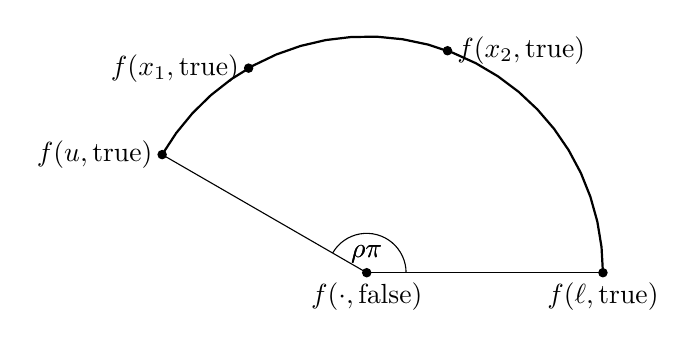
\begin{tikzpicture}

\pgfmathsetlengthmacro{\r}{3cm}
	\coordinate (O) at (0, 0);
	\coordinate (left) at ({3*cos(150)}, {3*sin(150)});

	\coordinate (right) at (\r, 0);
	\coordinate (x1) at ({3*cos(120)}, {3*sin(120)});
	\coordinate (x2) at ({3*cos(70)}, {3*sin(70)});

	% Draw big arc	
	\draw [black,thick,domain=0:150] plot ({3*cos(\x)}, {3*sin(\x)});

	\draw[fill] (left) circle (1.5pt);
	\draw (left) node[below, left] {$f(u, \textnormal{true})$};
	
	\draw[fill] (right) circle (1.5pt);
	\draw (right) node[below] {$f(\ell, \textnormal{true})$};

	\draw[fill] (O) circle (1.5pt);
	\draw (O) node[below] {$f(\cdot, \textnormal{false})$};

	\draw[fill] (x1) circle (1.5pt);
	\draw (x1) node[above, left] {$f(x_1, \textnormal{true})$};

	\draw[fill] (x2) circle (1.5pt);
	\draw (x2) node[above, right] {$f(x_2, \textnormal{true})$};
	
	% Draw little arc to denote the angle
	\draw (left) -- (O) node[above] {$\rho \pi$};
	\draw (right) -- (O) node[above] {$\rho \pi$};
	\draw [black,domain=0:150] plot ({0.5*cos(\x)}, {0.5*sin(\x)});
	
  \end{tikzpicture}
\end{center}
\caption{A demonstration of the embedding giving rise to the pseduo-metric: All points for which $\delta_i(x) =$ false are mapped to the same point.  Points for which $\delta_i(x) =$ true are mapped to a semicircle.  This embedding gives a constant distance between pairs of points which have differing values of $\delta$.  The parameter $\rho$ determines how much distance there is along the arc.}
\end{figure}




Let's first focus on a bounded real input dimension $i$, i.e., $\sX_i=[l_i, u_i]$.
To emphasize that we're in this real case, we explicitly denote the pseudometric as $d\br_i$ and the (pseudo-)isometry from $(\sX, d_i)$ to $\reals^2,d_\text{E}$ 
as $f\br_i$. For the definitions, recall that $\delta_i(\v{x})$ is true iff dimension $i$ is active given the instantiation of $i$'s ancestors in $\v{x}$.

\begin{eqnarray}
\nonumber{}d\br_i(\v{x}, \v{x}') & = & \left\{\begin{array}{ll}
\nonumber{} 0 & \textrm{ if } \delta_i(\v{x}) = \delta_i(\v{x}') = \textrm{false}\\
\nonumber{} \omega_i & \textrm{ if } \delta_i(\v{x}) \neq \delta_i(\v{x}')\\
\nonumber{} \omega_i \sqrt{2} \sqrt{1 - \cos(\pi\rho_i \frac{x_i-x_i'}{u_i-l_i})} & \textrm{ if } \delta_i(\v{x}) = \delta_i(\v{x}') = \textrm{true}. \end{array}\right.
\end{eqnarray}

\begin{eqnarray}
\nonumber{}f_i\br(\v{x}) & = & \left\{\begin{array}{ll}
[0,0]^\transpose & \textrm{ if } \delta_i(\v{x}) = \textrm{ false }\\
\nonumber{} \omega_i [\sin{\pi\rho_i\frac{x_i}{u_i-l_i}}, \cos{\pi\rho_i\frac{x_i}{u_i-l_i}}]^\transpose & \textrm{ otherwise.}\end{array}\right..
\end{eqnarray}

Although our formal arguments do not rely on this, Proposition \ref{prop:dbr_pseudometric} in the appendix shows that $d\br_i$ is a pseudometric. 
This pseudometric is defined by two parameters: $\omega_i \in [0,1]$ and $\rho_i \in [0,1]$. We firstly define 
\begin{equation}\label{eq:gamma}
\omega_i = \prod_{j \in \text{anc}_i \cup \{i\}} \gamma_j, 
\end{equation}
where $\gamma_j \in [0,1]$. This encodes the intuitive notion that differences on lower levels of the hierarchy count less than differences in their ancestors.

Also note that, as desired, if $i$ is inactive for both $\v{x}$ and $\v{x}'$, $d\br_i$ specifies that $g(\v{x})$ and $g(\v{x}')$ should not differ owing to differences between $x_i$ and $x_i'$. Secondly, if $i$ is active for both $\v{x}$ and $\v{x}'$, the difference between $g(\v{x})$ and $g(\v{x}')$ due to $x_i$ and $x_i'$ increases monotonically with increasing $\left|x_i-x_i'\right|$. Parameter $\rho_i$ controls whether differing in the activity of $i$ contributes more or less to the distance than differing in $x_i$ should $i$ be active. If $\rho = \nicefrac{1}{3}$, and if $i$ is inactive for exactly one of $\v{x}$ and $\v{x}'$, $g(\v{x})$ and $g(\v{x}')$ are as different as is possible due to dimension $i$; that is, $g(\v{x})$ and $g(\v{x}')$ are exactly as different in that case as if $x_i=l_i$ and $x_i'=u_i$. For $\rho>\nicefrac{1}{3}$, $i$ being active for both $\v{x}$ and $\v{x}'$ means that $g(\v{x})$ and $g(\v{x}')$ could potentially be more different than if
$i$ was active in only one of them. For $\rho<\nicefrac{1}{3}$, the converse is true.\footnote{Note that $\v{x}$ and $\v{x}'$ must differ in at least one ancestor dimension of $i$ in order for $\delta_i(\v{x}) \neq \delta_i(\v{x}')$ to hold, such that in the final kernel combining kernels $k_i$ due to each dimension $i$, differences in the activity of dimension $i$ are penalized both in kernel $k_i$ and in the distance for the kernel of the ancestor dimension causing the difference in $i$'s activity.}
%\note{FH: note: if we wanted to, we could probably get a condition for the joint overall kernel that the distance will always be larger if configurations differ on a higher level in the dimensionality DAG, by multiplying $\omega_i$ by the weights $\omega_j \in [0,1]$ of all of $i$'s ancestors $j$ (because at least one ancestor has to differ). We'd further have to divide $\omega_i$ by the maximal number of descendants a dimension has, in order to ensure that a difference at a higher level counts more than all the differences at the descendant-dimensions combined. But of course for this we wouldn't be able to do the proof of PSD-ness for each dimension by itself, so things would get a lot more hairy, and at least at this point there is no need for that.\\MO: actually, we should absolutely be able to do that, without any problem. I don't think it'll get hairy. It's just a matter of replacing $\omega_i$ with a slightly different constant, dependent on $i$, but independent of $\v{x}$. Let's do it!\\FH: I agree with what you did, and it's nice! What I actually meant would be hairy is to not penalize differences in activity of $i$ at all on the level of $i$, but to do it all on the ancestor level. For that each individual dimension would not define a kernel anymore, so the current way of proving PSD-ness wouldn't work anymore, and in general, thinking more about it now, the end result might not even be PSD. But enough of me going on about this, what we have now is nice :-) Please feel free to delete the note ...}

We now show that $d\br_i$ and $f\br_i$ can be plugged into a positive semi-definite kernel over Euclidean space to define a valid kernel over space $\sX$.

\begin{prop}
Let $\kappa$ be a positive semi-definite covariance function over Euclidean space.
Then, $k_i\colon \sX \times \sX\to \reals^+$, defined by 
%\[k_i(\v{x},\v{x}') = \kappa( d_{\text{E}}(f_i(\v{x}), f_i(\v{x}')) )\]
\[k_i(\v{x},\v{x}') = \kappa\bigl( d\br_i(\v{x}, \v{x}') \bigr)\]
is a positive semi-definite covariance function over input space $\sX$. 
\label{prop:cont_psd}
\begin{proof}
Due to Proposition \ref{prop:psd_if_isometry}, we only need to show that, for any two inputs $\v{x},\v{x}' \in \sX$, the isometry condition $d_{\text{E}}\bigl(f_i\br(\v{x}),f_i\br(\v{x}')\bigr) = d\br_i(\v{x},\v{x}')$ holds.

We use the abbreviation $\alpha = \pi\rho_i\frac{x_i}{u_i-l_i}$ and $\alpha' = \pi\rho_i\frac{x'_i}{u_i-l_i}$ and consider the following three possible cases of dimension $i$ being active or inactive in $\v{x}$ and $\v{x}'$.

~\\\noindent{}{Case 1}: $\delta_i(\v{x}) = \delta_i(\v{x}') = \textrm{false}$.
In this case, we trivially have 
\[d_{\text{E}}(f_i\br(\v{x}),f_i\br(\v{x}')) = d_{\text{E}}([0,0]^\transpose, [0,0]^\transpose) = 0 = d\br_i(\v{x},\v{x}').\]

~\\\noindent{}{Case 2}: $\delta_i(\v{x}) \neq \delta_i(\v{x}')$. In this case, we have
\[d_{\text{E}}(f_i\br(\v{x}),f_i\br(\v{x}')) = d_{\text{E}}([\sin{\alpha}, \cos{\alpha}]^\transpose, [0,0]^\transpose) = \sqrt{\omega_i^2 (\sin^2{\alpha} + \cos^2{\alpha})} = \omega_i = d\br_i(\v{x},\v{x}'),\]
and symmetrically for $d_{\text{E}}([0,0]^\transpose, [\sin{\alpha}, \cos{\alpha}]^\transpose)$.

~\\\noindent{}{Case 3}: $\delta_i(\v{x}) = \delta_i(\v{x}') = \textrm{true}$. We have:
\begin{eqnarray}
\nonumber{}d_{\text{E}}(f_i\br(\v{x}),f_i\br(\v{x}')) & = & d_{\text{E}}(\omega_i [\sin{\alpha}, \cos{\alpha}]^\transpose, \omega_i [\sin{\alpha'}, \cos{\alpha'}]^\transpose)\\ 
\nonumber{}& = & \omega_i \sqrt{(\sin{\alpha}-\sin{\alpha'})^2+ (\cos{\alpha}-\cos{\alpha'})^2}\\
\nonumber{}& = & \omega_i \sqrt{\sin^2{\alpha} -2 \sin{\alpha}\sin{\alpha'} + \sin^2{\alpha'}  + \cos^2{\alpha} -2 \cos{\alpha}\cos{\alpha'} + \cos^2{\alpha'} }\\
\nonumber{}& = & \omega_i \sqrt{(\sin^2{\alpha}+\cos^2{\alpha})   +  (\sin^2{\alpha'}+\cos^2{\alpha'})   -2 (\sin{\alpha}\sin{\alpha'} + \cos{\alpha}\cos{\alpha'})}\\
\label{eqn:simplified}& = & \omega_i \sqrt{ 1+1-2 \cos(\alpha-\alpha')}\\
\nonumber& = & \omega_i \sqrt{2} \sqrt{1 - \cos(\pi\rho_i \frac{x_i-x_i'}{u_i-l_i})} = d\br_i(\v{x}, \v{x}'),
\end{eqnarray}
where (\ref{eqn:simplified}) follows from the previous line by using the identity 
\[\cos{(a-b)} = \cos{a}\cos{b} + \sin{a}\sin{b}.\]
\end{proof}
\end{prop}












% \hide{
% %MO: older, simpler version hid
% %%%%%%%%%%%%%%%%%%%%%%%%%%%%%%%%%%%%%%%%%%%%%%%%%%%%%%%%%%%%%%%%%%%%%%%%%%%%%%%%%%%%%%%%%%%%%%%%%%%%%%%%%%%%%%%%%%%%%%%%%%%%%
% \section{Categorical Dimensions}
% %%%%%%%%%%%%%%%%%%%%%%%%%%%%%%%%%%%%%%%%%%%%%%%%%%%%%%%%%%%%%%%%%%%%%%%%%%%%%%%%%%%%%%%%%%%%%%%%%%%%%%%%%%%%%%%%%%%%%%%%%%%%%
% 
% Now let's define $f\cat_i$ and $d\cat_i$ for the case that the input $\sX_i=\{v_{i,1}, \dots, v_{i,m_i}\}$ is categorical with $m_i$ possible values. 
% Proceeding as above, we define a pseudometric $d\cat_i$ on $\sX$ and an isometry from $(\sX, d\cat_i)$ to $(\reals^{m_i},d_{\text{E}}^{m_i})$, and show that we can combine these
% with a kernel over Euclidean space to construct a valid kernel over space $\sX$. 
% 
% \begin{eqnarray}
% \nonumber{}d\cat_i(\v{x}, \v{x}') & = & \left\{
% \begin{array}{ll}
% \nonumber{} 0 & \textrm{ if } \delta_i(\v{x}) = \delta_i(\v{x}') = \textrm{false}\\
% \nonumber{} w_i & \textrm{ if } \delta_i(\v{x}) \neq \delta_i(\v{x}')\\
% \nonumber{} w_i \sqrt{2} \indicator_{x_i \neq x_i'} 
% & \textrm{ if } \delta_i(\v{x}) = \delta_i(\v{x}') = \textrm{true}.
% \end{array}
% \right.
% \end{eqnarray}
% 
% \begin{eqnarray}
% \nonumber{}f\cat_i(\v{x}) & = & \left\{\begin{array}{ll}
% \v{0} \in \reals^{m_i} & \textrm{ if } \delta_i(\v{x}) = \textrm{ false }\\
% \nonumber{} w_i\,\v{e_j} & \delta_i(\v{x}) = \textrm{ true and } x_i = v_{i,j},
% \end{array}\right.
% \end{eqnarray}
% \noindent{}where $\v{e_j} \in \reals^{m_i}$ is the $j$th unit vector: zero in all dimensions except $j$, where it is $1$.
% 
% Again, although our analysis does not rely on the fact, we prove in Proposition \ref{
% 
% {eq:gamma}
% 
% \begin{prop}
% Let $\kappa$ be a positive semi-definite covariance function over Euclidean space.
% Then, $k_i\colon \sX \times \sX\to \reals^+$, defined by 
% %\[k_i(\v{x},\v{x}') = \kappa( d_{\text{E}}(f_i(\v{x}), f_i(\v{x}')) )\]
% \[k_i(\v{x},\v{x}') = \kappa\bigl( d\cat_i(\v{x}, \v{x}') \bigr)\]
% is a positive semi-definite covariance function over input space $\sX$. 
% \label{prop:cat_psd}
% \begin{proof}
% We proceed as in the proof of Proposition \ref{prop:cont_psd} to show that, for any two inputs $\v{x},\v{x}' \in \sX$, the isometry condition $d_{\text{E}}^{m_i}(f\cat_i(\v{x}),f\cat_i(\v{x}')) = d\cat_i(\v{x},\v{x}')$ holds.
% 
% ~\\\noindent{}{Case 1}: $\delta_i(\v{x}) = \delta_i(\v{x}') = \textrm{false}$.
% In this case, we trivially have 
% \[d_{\text{E}}^{m_i}(f_i\br(\v{x}),f_i\br(\v{x}')) = d_{\text{E}}^{m_i}(\v{0}, \v{0}) = 0 = d_i\br(\v{x},\v{x}').\]
% 
% ~\\\noindent{}{Case 2}: $\delta_i(\v{x}) \neq \delta_i(\v{x}')$. In this case, we have
% \[d_{\text{E}}^{m_i}(f\cat_i(\v{x}),f\cat_i(\v{x}')) = d_{\text{E}}^{m_i}(w_i\,\v{e_j}, \v{0}) = w_i = d_i(\v{x},\v{x}'),\]
% and symmetrically for $d_{\text{E}}(\v{0}, w_i\,\v{e_j})$.
% 
% ~\\\noindent{}{Case 3}: $\delta_i(\v{x}) = \delta_i(\v{x}') = \textrm{true}$. 
% If $x_i=x_i'=v_{i,j}$, we have 
% \begin{eqnarray}
% \nonumber{}d_{\text{E}}^{m_i}(f\cat_i(\v{x}),f\cat_i(\v{x}')) & = & d_{\text{E}}^{m_i}(w_i\,\v{e_j}, w_i\,\v{e_j}) = 0 = d\cat_i(\v{x}, \v{x}')
% \end{eqnarray}
% 
% \noindent{}If $x_i=v_{i,j} \neq v_{i,j'} = x_i'$, we have 
% \begin{eqnarray} 
% \nonumber{}d_{\text{E}}(f\cat_i(\v{x}),f\cat_i(\v{x}')) & = & d_{\text{E}}^{m_i}(w_i\,\v{e_j}, w_i \v{e_{j'}}) = w_i \sqrt{2} = d\cat_i(\v{x}, \v{x}')
% \end{eqnarray}
% \end{proof}
% \end{prop}
% }







%%%%%%%%%%%%%%%%%%%%%%%%%%%%%%%%%%%%%%%%%%%%%%%%%%%%%%%%%%%%%%%%%%%%%%%%%%%%%%%%%%%%%%%%%%%%%%%%%%%%%%%%%%%%%%%%%%%%%%%%%%%%%
\section{Categorical Dimensions}
%%%%%%%%%%%%%%%%%%%%%%%%%%%%%%%%%%%%%%%%%%%%%%%%%%%%%%%%%%%%%%%%%%%%%%%%%%%%%%%%%%%%%%%%%%%%%%%%%%%%%%%%%%%%%%%%%%%%%%%%%%%%%

Now let's define $f\cat_i$ and $d\cat_i$ for the case that the input $\sX_i=\{v_{i,1}, \dots, v_{i,m_i}\}$ is categorical with $m_i$ possible values. 
Proceeding as above, we define a pseudometric $d\cat_i$ on $\sX$ and an isometry from $(\sX, d\cat_i)$ to $(\reals^{m_i},d_{\text{E}}^{m_i})$, and show that we can combine these
with a kernel over Euclidean space to construct a valid kernel over space $\sX$. 

\begin{eqnarray}
\nonumber{}d\cat_i(\v{x}, \v{x}') & = & \left\{
\begin{array}{ll}
\nonumber{} 0 & \textrm{ if } \delta_i(\v{x}) = \delta_i(\v{x}') = \textrm{false}\\
\nonumber{} \omega_i & \textrm{ if } \delta_i(\v{x}) \neq \delta_i(\v{x}')\\
\nonumber{} \omega_i \frac{\sqrt{2} \rho}
{1+(m_i-1)(1-\rho)^2}
 \indicator_{x_i \neq x_i'} 
& \textrm{ if } \delta_i(\v{x}) = \delta_i(\v{x}') = \textrm{true}.
\end{array}
\right.
\end{eqnarray}

\begin{eqnarray}
\nonumber{}f\cat_i(\v{x}) & = & \left\{\begin{array}{ll}
\v{0} \in \reals^{m_i} & \textrm{ if } \delta_i(\v{x}) = \textrm{ false }\\
\nonumber{} \omega_i\,\frac{\v{e_j}+(1-\rho)\sum_{l\neq j} \v{e_l}}
{\sqrt{1+(m_i-1)(1-\rho)^2}}
 & \textrm{ if } \delta_i(\v{x}) = \textrm{ true and } x_i = v_{i,j},
\end{array}\right.
\end{eqnarray}
\noindent{}where $\v{e_j} \in \reals^{m_i}$ is the $j$th unit vector: zero in all dimensions except $j$, where it is $1$. Note that
\begin{equation}
 \sqrt{1+(m_i-1)(1-\rho)^2} = \biggl\|\v{e_j}+(1-\rho)\sum_{l\neq j} \v{e_l}\biggr\|.
\end{equation}

\noindent{}Again, although our analysis does not require it, we prove in Proposition \ref{prop:dbr_pseudometric_cat} (see appendix) that $d\cat_i$ is a pseudometric. Our pseudometric is again defined by two hyperparameters. Firstly, $\omega_i\in[0,1]$ is exactly as defined in \eqref{eq:gamma}, and similarly allows higher-level inputs to attain greater importance. Similarly, $\rho_i\in[0,1]$ allows control of to what extent differing in the activity of $i$ affects the distance relative to the influence of differing in $x_i$ should $i$ be active. In particular, for
\begin{equation}
 \rho_i^\ast = 
\frac{\sqrt{2}-2+2m_i-\sqrt{6-4\sqrt{2}+4(\sqrt{2}-1)m_i}}
{2(m_i-1)},
\end{equation}
$\rho_i<\rho_i^\ast$ implies that differing in the activity of $i$ is more significant, whereas $\rho_i>\rho_i^\ast$ implies the converse. The special case $\rho = 0$ dictates that differing in $x_i$ has no influence on the distance; $\rho=1$ assigns maximal importance to differing in $x_i$. 

\begin{prop}
Let $\kappa$ be a positive semi-definite covariance function over Euclidean space.
Then, $k_i\colon \sX \times \sX\to \reals^+$, defined by 
%\[k_i(\v{x},\v{x}') = \kappa( d_{\text{E}}(f_i(\v{x}), f_i(\v{x}')) )\]
\[k_i(\v{x},\v{x}') = \kappa\bigl( d\cat_i(\v{x}, \v{x}') \bigr)\]
is a positive semi-definite covariance function over input space $\sX$. 
\label{prop:cat_psd}
\begin{proof}
We proceed as in the proof of Proposition \ref{prop:cont_psd} to show that, for any two inputs $\v{x},\v{x}' \in \sX$, the isometry condition $d_{\text{E}}^{m_i}(f\cat_i(\v{x}),f\cat_i(\v{x}')) = d\cat_i(\v{x},\v{x}')$ holds.

~\\\noindent{}{Case 1}: $\delta_i(\v{x}) = \delta_i(\v{x}') = \textrm{false}$.
In this case, we trivially have 
\[d_{\text{E}}^{m_i}(f_i\br(\v{x}),f_i\br(\v{x}')) = d_{\text{E}}^{m_i}(\v{0}, \v{0}) = 0 = d_i\br(\v{x},\v{x}').\]

~\\\noindent{}{Case 2}: $\delta_i(\v{x}) \neq \delta_i(\v{x}')$. In this case, we have
\[d_{\text{E}}^{m_i}(f\cat_i(\v{x}),f\cat_i(\v{x}')) = 
d_{\text{E}}^{m_i}\biggl(\omega_i\,\frac{\v{e_j}+(1-\rho)\sum_{l\neq j} \v{e_l}}
{\|\v{e_j}+(1-\rho)\sum_{l\neq j} \v{e_l}\|}, \v{0}\biggr) 
= \omega_i = d_i(\v{x},\v{x}'),\]
and symmetrically for $d_{\text{E}}\biggl(\v{0}, \omega_i\,\frac{\v{e_j}+(1-\rho)\sum_{l\neq j} \v{e_l}}
{\|\v{e_j}+(1-\rho)\sum_{l\neq j} \v{e_l}\|}\biggr)$.

~\\\noindent{}{Case 3}: $\delta_i(\v{x}) = \delta_i(\v{x}') = \textrm{true}$. 
If $x_i=x_i'=v_{i,j}$, we have 
\begin{eqnarray}
\nonumber{}d_{\text{E}}^{m_i}(f\cat_i(\v{x}),f\cat_i(\v{x}')) & = & d_{\text{E}}^{m_i}\bigl(
f\cat_i(\v{x}),f\cat_i(\v{x})
\bigr) = 0 = d\cat_i(\v{x}, \v{x}').
\end{eqnarray}

\noindent{}If $x_i=v_{i,j} \neq v_{i,j'} = x_i'$, we have 
\begin{align} 
\nonumber{}d_{\text{E}}(f\cat_i(\v{x}),f\cat_i(\v{x}')) & = 
d_{\text{E}}^{m_i}\biggl(
\omega_i\,\frac{\v{e_j}+(1-\rho)\sum_{l\neq j} \v{e_l}}
{\sqrt{1+(m_i-1)(1-\rho)^2}},\,
\omega_i\,\frac{\v{e_j'}+(1-\rho)\sum_{l\neq j'} \v{e_l}}
{\sqrt{1+(m_i-1)(1-\rho)^2}}
\biggr) \\
& = \omega_i \frac{\sqrt{\bigl(1-(1-\rho)\bigr)^2 + \bigl(1-(1-\rho)\bigr)^2}}
{1+(m_i-1)(1-\rho)^2} \nonumber\\
& = \omega_i \frac{\sqrt{2} \rho}
{1+(m_i-1)(1-\rho)^2} \nonumber\\
& = d\cat_i(\v{x}, \v{x}').
\end{align}
\end{proof}
\end{prop}

\section{Experiments}

All the separate models split the data into 6 different datasets, one for each level, and build a separate model for each level.  The gp-hierarchical model gets all the data together because it can handle it.  

However, The gp-hierarchical model changes two things at once compared to the separate-gp-ard model: besides embedding the missing data in a different spot, it also has embeds the fully-observed data on semi-circles, and has a different parameterization.  
So, it could be the case that even when the data are fully observed, embedding the data on a semi-circle and using a different parameterization might cause better or worse performance than a standard squared-exp.  To find out if this is the case, we compare separate-gp-ard and separate-hierarchical to find out if these two models have different performance even in the standard fully-observed case.

% --- Automatically generated by resultsToLatex4.m ---
% Exported at 15-Jan-2014 16:15:50
\begin{center}
\begin{tabular}{l | r r r r r r}
Method & \rotatebox{0}{ NN   }  & \rotatebox{0}{ NN   log }  & \rotatebox{0}{ NN   half }  & \rotatebox{0}{ NN   log half }  & \rotatebox{0}{ concrete 500 }  & \rotatebox{0}{ housing }  \\ \hline
Separate Linear & $0.898$ & $0.874$ & $0.982$ & $\mathbf{3.482}$ & $\mathbf{ NaN}$ & $\mathbf{ NaN}$ \\
Separate {\sc gp} & $0.815$ & $0.547$ & $1.012$ & $0.753$ & $\mathbf{ NaN}$ & $\mathbf{ NaN}$ \\
Poor Man's embedding Linear & $0.882$ & $0.661$ & $0.980$ & $0.732$ & $0.403$ & $\mathbf{0.388}$ \\
Poor Man's embedding {\sc gp} & $\mathbf{0.787}$ & $\mathbf{0.498}$ & $0.819$ & $0.656$ & $\mathbf{0.164}$ & $\mathbf{0.284}$ \\
Separate Hierarchical {\sc gp} & $0.771$ & $0.554$ & $\mathbf{0.983}$ & $0.847$ & $\mathbf{ NaN}$ & $\mathbf{ NaN}$ \\
Hierarchical {\sc gp} & $0.744$ & $\mathbf{0.450}$ & $\mathbf{0.674}$ & $\mathbf{0.607}$ & $1.217$ & $\mathbf{0.411}$ \\
sep box & $\mathbf{0.687}$ & $\mathbf{0.519}$ & $\mathbf{0.753}$ & $\mathbf{0.598}$ & $\mathbf{ NaN}$ & $\mathbf{ NaN}$ \\
gp box & $\mathbf{0.621}$ & $\mathbf{0.485}$ & $\mathbf{0.675}$ & $\mathbf{0.575}$ & $0.836$ & $1.087$ \\
\end{tabular}
\end{center}
% End automatically generated LaTeX



\appendix

\section{Proof of pseudometric properties}

\begin{prop}
  $d\br_i$ is a pseudometric on $\sX$. \label{prop:dbr_pseudometric}
\begin{proof}
The non-negativity and symmetry of $d\br_i$ are trivially proven. To prove the triangle inequality, consider $\v{x}, \v{x}', \v{x}'' \in \sX$. 

~\\\noindent{}{Case 1}: $\delta_i(\v{x}) = \delta_i(\v{x}') = \textrm{false}$, such that $d\br_i(\v{x},\v{x}') = 0$. Here, from non-negativity, clearly $d\br_i(\v{x},\v{x}') = 0 \leq d\br_i(\v{x},\v{x}'') + d\br_i(\v{x}',\v{x}'')$.

~\\\noindent{}{Case 2}: $\delta_i(\v{x}) \neq \delta_i(\v{x}')$, such that such that  $d\br_i(\v{x},\v{x}') = \omega_i$.  Without loss of generality, assume $\delta_i(\v{x}) = \text{true}$, $\delta_i(\v{x}') = \text{false}$ and $\delta_i(\v{x}'') = \text{true}$. 
\begin{align}
d\br_i(\v{x},\v{x}'') + d\br_i(\v{x}',\v{x}'') = d\br_i(\v{x},\v{x}'')  + \omega_i
\end{align}
Hence $d\br_i(\v{x},\v{x}'') + d\br_i(\v{x}',\v{x}'') \geq \omega_i = d\br_i(\v{x},\v{x}')$ by non-negativity.

~\\\noindent{}{Case 3}: $\delta_i(\v{x}) = \delta_i(\v{x}')=\textrm{true}$, such that  $d\br_i(\v{x},\v{x}') = \omega_i \sqrt{2} \sqrt{1 - \cos(\pi\rho_i \frac{x_i-x_i'}{u_i-l_i})}$.  If  $\delta_i(\v{x}'') = \text{false}$,
\begin{align}
d\br_i(\v{x},\v{x}'') + d\br_i(\v{x}',\v{x}'') = 2 \omega_i \geq \omega_i \sqrt{2} \sqrt{1 - \cos(\pi\rho_i \frac{x_i-x_i'}{u_i-l_i})} = d\br_i(\v{x},\v{x}').
\end{align} 
If  $\delta_i(\v{x}'') = \text{true}$, consider the `worst' possible case in which, without loss of generality, $x_i=l_i$ and $x'_i=u_i$, such that $d\br_i(\v{x},\v{x}')=2 \omega_i^2$.  We define the abbreviation $\beta'' = \frac{x''_i-l_i}{u_i-l_i}$, giving
\begin{align}
\bigl(d\br_i(\v{x},\v{x}'') + d\br_i(\v{x}',\v{x}'')\bigr)^2
& = 2\omega_i^2 \Bigl(\sqrt{1 - \cos (\pi\rho_i \beta'')} + \sqrt{1 - \cos \bigl(\pi\rho_i (1-\beta'')\bigr)}\Bigr)^2\nonumber\\
&=2\omega_i^2\biggl(2 - \cos (\pi\rho_i \beta'') - \cos \bigl(\pi\rho_i (1-\beta'')\bigr)
\nonumber\\
&\qquad\qquad+2\sqrt{\Bigl(1 - \cos (\pi\rho_i \beta'')\Bigr)\Bigl(1 - \cos \bigl(\pi\rho_i (1-\beta'')\bigr)\Bigr)}\biggr)\nonumber\\
&=2\omega_i^2\biggl(2 +2\sqrt{1 + \cos (\pi\rho_i \beta'')\cos \bigl(\pi\rho_i (1-\beta'')\bigr)}\biggr)\nonumber\\
&=4 \omega_i^2 \bigl(1 + \left|\sin \pi\rho_i \beta'' \right|\bigr)\nonumber\\
&\geq 4 \omega_i^2 = d\br_i(\v{x},\v{x}')^2.
\end{align}
Hence, from non-negativity, we have $d\br_i(\v{x},\v{x}'') + d\br_i(\v{x}',\v{x}'')\geq d\br_i(\v{x},\v{x}')$.
\end{proof}
\end{prop}

\begin{prop}
 $d\cat_i$ is a pseudometric on $\sX$.\label{prop:dbr_pseudometric_cat}
\begin{proof}
The non-negativity and symmetry of $d\cat_i$ are trivially proven. To prove the triangle inequality, consider $\v{x}, \v{x}', \v{x}'' \in \sX$. 

~\\\noindent{}{Case 1}: $\delta_i(\v{x}) = \delta_i(\v{x}') = \textrm{false}$, such that $d\cat_i(\v{x},\v{x}') = 0$. Here, from non-negativity, clearly $d\cat_i(\v{x},\v{x}') = 0 \leq d\cat_i(\v{x},\v{x}'') + d\cat_i(\v{x}',\v{x}'')$.

~\\\noindent{}{Case 2}: $\delta_i(\v{x}) \neq \delta_i(\v{x}')$, such that such that  $d\cat_i(\v{x},\v{x}') = \omega_i$.  Without loss of generality, assume $\delta_i(\v{x}) = \text{true}$, $\delta_i(\v{x}') = \text{false}$ and $\delta_i(\v{x}'') = \text{true}$. 
\begin{align}
d\cat_i(\v{x},\v{x}'') + d\cat_i(\v{x}',\v{x}'') = d\cat_i(\v{x},\v{x}'')  + \omega_i
\end{align}
Hence $d\cat_i(\v{x},\v{x}'') + d\cat_i(\v{x}',\v{x}'') \geq \omega_i = d\cat_i(\v{x},\v{x}')$ by non-negativity.

~\\\noindent{}{Case 3}: $\delta_i(\v{x}) = \delta_i(\v{x}')=\textrm{true}$, such that  $d\cat_i(\v{x},\v{x}') =
\omega_i \frac{\sqrt{2} \rho}
{1+(m_i-1)(1-\rho)^2}
 \indicator_{x_i \neq x_i'} $.  
If  $\delta_i(\v{x}'') = \text{false}$,
\begin{align}
d\cat_i(\v{x},\v{x}'') + d\cat_i(\v{x}',\v{x}'') = 
2 \omega_i 
\geq 
\omega_i \frac{\sqrt{2} \rho}
{1+(m_i-1)(1-\rho)^2}
 \indicator_{x_i \neq x_i'}  
= d\cat_i(\v{x},\v{x}').
\end{align} 
If  $\delta_i(\v{x}'') = \text{true}$, 
\begin{align}
d\cat_i(\v{x},\v{x}'') + d\cat_i(\v{x}',\v{x}'')
& = \omega_i \frac{\sqrt{2} \rho}
{1+(m_i-1)(1-\rho)^2}
(
 \indicator_{x_i \neq x_i''} 
+
 \indicator_{x_i' \neq x_i''} 
)
\nonumber\\
& \geq 
\omega_i \frac{\sqrt{2} \rho}
{1+(m_i-1)(1-\rho)^2}
 \indicator_{x_i \neq x_i'} = d\cat_i(\v{x},\v{x}').
\end{align}
\end{proof}
\end{prop}

%\bibliographystyle{theapa}
%\renewcommand{\baselinestretch}{0.97}
%\footnotesize{\bibliography{abbrev,frankbib}}

\cite{rasmussen38gaussian}

\bibliography{hierarchicalkernel}
\bibliographystyle{unsrt}


\end{document}

